\documentclass{article}
\usepackage{color}
\usepackage{multirow}
\usepackage{moreverb}
\usepackage{bigbox}
\usepackage{rotating}
\usepackage{verbatim}
\usepackage{graphicx}
\usepackage{fullpage}
\usepackage{url}

\bibliographystyle{elsart-num}
\setlength{\linewidth}{5pt}

\begin{document}

\title{Surfpack User's Manual \\ Version 1.1}

\author{Keith R. Dalbey$^1$, Anthony A. Giunta$^1$, Mark D. Richards$^2$, Eric C. Cyr$^1$ \\Laura P. Swiler$^1$, Shane L. Brown$^1$, Michael S. Eldred$^1$, Brian M. Adams$^1$}

\maketitle


\begin{center}
$^1$Sandia National Laboratories*\\P.O. Box 5800, Mail Stop 1318\\Albuquerque, NM 87185-1318 USA \\
Email: surfpack-developers@development.sandia.gov \\ Web: http://dakota.sandia.gov/packages/surfpack
\end{center}

\bigbreak

\begin{center}
$^2$University of Illinois at Urbana-Champaign\\Dept. of Computer Science\\201 North Goodwin Ave.\\Urbana, IL 61801-2302 USA\\
Web: http://cs.engr.uiuc.edu
\end{center}

\bigbreak

\begin{center}
Copyright 2006, Sandia National Laboratories
\end{center}

\bigbreak

\begin{center}
*Sandia is a multiprogram laboratory operated by Sandia Corporation, a Lockheed Martin Company, 
for the United States Department of Energy's National Nuclear Security Administration under 
contract DE-AC04-94AL85000.
\end{center}

\pagebreak

\section {Overview}\label{sec:overview}
Surfpack is a collection of surface-fitting methods and accompanying metrics to evaluate or predict the quality of the generated surfaces.  The concept of creating a global approximation or ``fit'' from a collection of data samples is utilized in many scientific disciplines, but the nomenclature varies widely from field to field.  The results from the application of such methods are commonly called empirical models, response surfaces, surrogate models, function approximations, or meta-models.  Many different algorithms have been developed to generalize from a set of data; these algorithms have different strengths and weaknesses.  The goals of Surfpack are

\begin{enumerate}
\item to give users the option to use any of several methods, depending on the nature of the specific application; and
\item to put data-fitting methods that are commonly used in various disciplines into a common framework, where their properties can be more easily compared and analyzed.
\end{enumerate}
Surfpack's API includes a small set of commands, centered on the following general operations:
\begin{itemize}
\item {\bf Prepare a data set for use.}  This typically involves reading a formatted text file from disk.  Alternatively, the user may specify upper- and lower-bounds along one or more dimensions and generate a set of data points from those boundaries (either a grid or a set of Monte Carlo samples).
\item {\bf Create an empirical model from a set of data.} The user may choose one of several algorithms to create the surface approximation: Least-squares regression using polynomials, Multivariate Adaptive Regression Splines (MARS), Kriging interpolation, Artificial Neural Networks, Moving Least Squares, or Radial Basis Function Networks.
\item {\bf Evaluate an empirical model on a set of data.}  For the non-interpolating algorithms (e.g. polynomial regression), it may be of interest to evaluate the model at the same data sites that were used to generate it, to see how closely the model fits the data.  All of the algorithms all the user to evaluate the model at other data points where the true function value is not available.
\item {\bf Obtain measures of the ``goodness of fit'' of the model.}  Surfpack supports metrics such as mean squared error or maximum absolute error for data sets where the true function values are known.  Cross-validation metrics (e.g. PRESS) are also available for situations where all of the known data points for the function that is being approximated were used to create the empirical model.
\item {\bf Save the data and/or empirical models for future use.}  Data can be saved for later use, e.g., with a plotting package.  The approximating surfaces themselves may also be saved, so that a user can evaluate the model on a data set at a later time without having to recompute it.
\end{itemize}


\section{Installation}\label{sec:installation}
Surfpack is being developed primarily under Linux and is targeted to
all flavors of UNIX.  Platforms on which Surfpack has been
successfully built include Linux, SunOS, IRIX, OSF, AIX, Windows
(Cygwin), and Mac OS X.  Native Visual C++ compilation is not
currently supported.

\subsection{Obtaining Surfpack}
Surfpack source packages are distributed from
\url{http://dakota.sandia.gov/packages/surfpack}.  It is also included
in all Dakota distributions and can be obtained via anonymous
Subversion checkout from
\url{https://software.sandia.gov/svn/public/surfpack}.  Binary
packages are no longer supported.

\subsection{Requirements}
\begin{itemize}
\item {\bf C++}.  A majority of the source code for Surfpack is written in C++.  Surfpack makes frequent use of the standard C and C++ libraries, including the Standard Template Library.  The Kriging algorithm calls some FORTRAN code (pivoted Cholesky and some optimizers such as CONMIN).  
\item {\bf Fortran 77}.  The MARS algorithm is implemented in FORTRAN.  
\item {\bf BLAS}.  Many of the data-fitting algorithms rely on the Basic Linear Algebra Subroutines to perform rudimentary linear algebra operations.
\item {\bf LAPACK}.  Surfpack makes use of the following LAPACK~\cite{anderson}  driver routines: dpotrf, dpocon, dpotrs, dlange, dgetrf, dgetri, dgels, dgglse.  Implementations of LAPACK across different platforms seem to vary in terms of how many of these algorithms they support.  Therefore, source for these functions and their dependencies is included in the Surfpack distribution.  However, BLAS and LAPACK routines are usually highly optimized for each platform; performance is best when pre-compiled, native versions of these functions are available.
\end{itemize}
\subsection{Options}
\begin{itemize}
\item {\bf Boost serialization}.  As of Version 1.1, Surfpack's model save/load facility requires the Boost serialization binary component.
\item {\bf CPP Unit}.  A suite of unit tests is available on platforms where CPP Unit has been built.
\item {\bf lex and yacc}. Surfpack may be used as a library or as a stand-alone program.  The stand-alone executable requires lex and yacc (a lexical analyzer generator and parser generator, respectively), which are normally distributed with Unix-like operating systems.  They are also freely available on the Internet.
\end{itemize}

\subsection{Standard build}
To compile Surfpack from source, extract the source, configure with
CMake, and compile with your native make system, for example:
\begin{verbatim}
  tar xzf surfpack-1.1.tar.gz
  cd surfpack-1.1
  mkdir build && cd build
  cmake -DCMAKE_INSTALL_PREFIX=/apps/surfpack -DCMAKE_BUILD_TYPE=Release ..
  make -j 4
  [make install]
\end{verbatim}

\subsection{Testing the Installation}
\textit{Installation testing is not currently supported.}  Surfpack is
distributed with its test suite.  The unit testing suite utilizes the
CPP Unit libraries
(\url{http://www.sourceforge.net/projects/cppunit}), which must be
present if the tests are to be executed.  If the CPP Unit libraries
are installed in a location that is not automatically searched by the
compiler, the full path of the libraries should be specified as an
argument to \texttt{configure}:
\verbatimtabinput{Installation/configure_with_cppunit.txt} To run the
test suite, type \texttt{make check} at the command line, after the
successful execution of \texttt{make} or \texttt{make install}.  CPP
Unit summarize the results of the tests.

\section{Getting Started}
This chapter outlines the basic commands in the Surfpack API.  Normally, a script file
is passed to \texttt{surfpack} as a command-line argument; the commands in
the file are executed sequentially.  If no command-line arguments are given,
Surfpack reads a list of commands from standard input.

General conventions are presented in Section~\ref{sec:conventions}.  The various Surfpack commands
are discussed in Sections~\ref{sec:loaddata}--\ref{sec:saving} and are illustrated using the sample script \texttt{examples/GettingStarted/getting\_started.spk}.  

\subsection{Conventions}\label{sec:conventions}
Surfpack commands consist of a capitalized command name followed by a
comma-delimited list of arguments in square brackets \texttt{[ ]}.  Lines beginning with  `\#' are interpreted as comments and are ignored.  White-space is ignored inside commands. Lines beginning with `!' are passed along to the underlying shell.  (The
leading `!' is first removed.)  This allows the user to, for example, \texttt{echo}
information to the terminal or do pre- or post-processing on the data files.
Multiline shell commands are delimited by \texttt{/*} and \texttt{*/}.

The Surfpack interpreter internally maintains lists of three types of variables: \texttt{axes},
\texttt{data}, and \texttt{surfaces}.  Axes variables are created using the \texttt{CreateAxes}
command.  Data variables may be created by the \texttt{Load}, or \texttt{CreateSample}
commands.  Surfaces variables are created with the \texttt{Load} or
\texttt{CreateSurface} commands.  Any command that creates an \texttt{axes}, \texttt{data}, or \texttt{surface
}variable must have a \texttt{name} argument, so that the variable can be used in 
future commands.  When an existing variable is
used in a subsequent command, it is designated by an argument which names its
type (\texttt{axes}, \texttt{data}, or \texttt{surface}).  Figure~\ref{fig:conventions} shows examples of commands that create and/or use the different types of variables. 

\begin{figure}[htbp]
  \centering
  \begin{bigbox}
	\begin{small}
		\verbatimtabinput[8]{GettingStarted/conventions.txt}
 	\end{small}
  \end{bigbox}
  \caption{Examples showing the creation and usage of axes, data, and surface variables.  The file, \texttt{conventions.spk}, is located in the \texttt{examples/GettingStarted} subdirectory.}
   \label{fig:conventions}
\end{figure}

\subsubsection{Command Arguments}\label{sec:arguments}

Each argument has the format \texttt{argument\_name =
argument\_value}.  An argument name is an identifier:  a letter followed by a
combination of letters, digits, and underscores.  An
argument value may be an identifier, an integer or
real-valued number, a string literal (enclosed in single quotes ` '), or a comma-separated list of values enclosed in parentheses,
{\em e.g.}, \texttt{(1.0,3.5,4.0)}.  Arguments may appear in any order.

\subsection{Loading Data From a File}\label{sec:loaddata}
The first step in a Surfpack application is usually to prepare a data set for
future computation.  Typically, data have already been collected and are stored in a text file.  Surfpack requires data files to conform to a specific format.  The data points in the file should be listed one point per line.  Each point should consist of one or more predictor variables followed by zero or more response variables.  All data points in a single file must have the same number of variables; the variables for each point must appear in the same order.  An optional header line, beginning with a `\%', lists the labels for each of the variables.  Figure~\ref{fig:world_population} shows an example.
\begin{figure}[htbp]
  \centering
  \begin{bigbox}
	\begin{small}
		\verbatimtabinput[8]{GettingStarted/world_pop.spd}
 	\end{small}
  \end{bigbox}
  \caption{A data file containing ten data points with one predictor variable and seven response variables.  The file is \texttt{examples/GettingStarted/world\_pop.spd}.}
   \label{fig:world_population}
\end{figure}

Data files can be read into Surfpack using the \texttt{Load} command, which expects four arguments: a \texttt{name} identifier for the data set, a string argument \texttt{file} specifying the full or relative path of the data file, and integers \texttt{n\_predictors} and \texttt{n\_responses} which indicate the number of predictor and response variables, respectively, in the data set.  Surfpack expects data files to have a \texttt{.spd} extension.  The data set shown in Figure~\ref{fig:world_population} can be loaded into Surfpack using the following command:
\verbatimtabinput{GettingStarted/load.txt}

\subsection{Creating a model from existing data}\label{sec:create_surface}
The \texttt{CreateSurface} command creates a global approximation to a function using a sample of known points.  \texttt{CreateSurface} takes at least three
arguments: a \texttt{name} for the surface, the \texttt{data} from which the model is to be created, and the \texttt{type} of data-fitting algorithm.  Additional arguments may specify algorithm-specific parameters and/or data scaling options.  Consider the following command:
\verbatiminput{GettingStarted/create_surface.txt}
The \texttt{polynomial} value for the \texttt{type} argument tells Surfpack to use linear regression to fit the \texttt{world\_pop} data, which must have been created or loaded in a previous command.  The \texttt{order = 2} argument specifies that up to quadratic terms may be used in the regression model.  The \texttt{name} argument specifies that future commands may refer to this model as \texttt{world\_poly}.  The \texttt{response} parameter indicates which of the response variables in the \texttt{world\_poly} data set should be used to create the global approximation.  The \texttt{log\_scale} and \texttt{norm\_scale} arguments take parenthesized lists of variables that are to be scaled before the global approximation is created.  When a variable is scaled using \texttt{norm\_scale}, all of the values for that variable in the given data set are mapped to the interval $[0,1]$.

\subsection{Evaluating an existing model on a set of data}\label{sec:evaluate}

The \texttt{world\_pop} data set contains world population data from the years 1960--2005.  Suppose we wish to create a model to predict the size of the population at five year intervals up to 2050.  If a file with these query points already exists, it may be read in using the \texttt{Load} command as described above.  Alternatively, the data set may be created on the fly using Surfpack's \texttt{CreateAxes} and \texttt{CreateSample} commands.  The \texttt{CreateAxes} command defines minimum/maximum pairs for a list of variables on a Cartesian coordinate system.  These range pairs serve as the boundaries inside which future data sets may be created.  In this example, there is only one variable (time) and the range of values that we are interested in is $[2010,2050]$.  \texttt{CreateAxes} takes two arguments: normally a \texttt{name} identifier for the resulting \texttt{axes} variable that is created, and a string \texttt{bounds} that defines the boundaries for the data set.  For multidimensional data sets, the min/max pairs for each dimension should be delimited by '$|$'.  Since the population data set has only one predictor variable (year), the appropriate \texttt{CreateAxes} command is
\verbatimtabinput{GettingStarted/create_axes.txt}

With appropriate boundaries for our data set defined in an \texttt{axes} variable, we can use the \texttt{CreateSample} command to generate a set of query points.  \texttt{CreateSample} expects at least three arguments.  The \texttt{name} and \texttt{axes} identifiers give a designation and a reference to an existing \texttt{axes} variable, respectively, for the new data set.  For a random sampling of Monte Carlo points ({\em i.e.}, a data set where each variable for each point receives a random value drawn uniformly from the boundaries defined by the \texttt{axes} variable), the \texttt{size} argument specifies the number of points in the data set.  Alternatively, to generate regularly spaced points on a grid, the \texttt{grid\_points} argument is used.  The value for the \texttt{grid\_points} argument is a list of integers which specifies the number of grid points along each dimension.  The optional \texttt{labels} argument specifies a list of identifiers that are to be used as the headings for the variables in the new data set.  To generate query points at five-year intervals, we can use
\verbatiminput{GettingStarted/create_sample.txt}
  
Now we can use Surfpack's \texttt{Evaluate} command to make the predictions.  \texttt{Evaluate} takes two required parameters: a \texttt{surface} argument indicates which existing surface is to be  evaluated; a \texttt{data} argument gives the set of data that are to be evaluated.  Surfpack appends a new response variable to the data set.  An optional \texttt{label} argument gives a name for the new response:     
\verbatiminput{GettingStarted/evaluate.txt}

\subsection{Quantifying Model Fitness}\label{sec:fitness}
The quality of an approximation depends on the properties of
the function being approximated and on the data samples and algorithm used to
create the model.  Surfpack provides several metrics for quantifying how well
the model fits the data used to create it and for predicting how well the model
might generalize to unseen data.  These are accessible via the \texttt{Fitness} command,
which takes at least two arguments: the \texttt{surface} to be analyzed
and the quality-of-fit \texttt{metric} to be used:
\verbatiminput{GettingStarted/fitness.txt}
In this example, the mean squared error (MSE) for the \texttt{world\_poly} model is printed to the terminal.  Since we used a least-squares regression to fit the sample data points, our model is not guaranteed to match these ten points exactly ({\em i.e.}, the model's prediction at those points may not match the response values of the training data).
The difference between the model's prediction and the true response value is the {\em residual}.  The MSE is the arithmetic
mean of all the squared residuals.  MSE values near zero indicate a close fit of the model to the
training data.

\subsection{Saving the results of Surfpack computations}\label{sec:saving}
The \texttt{Save} command make it possible to store the results of Surfpack computations to files for inspection and future use.  The commands requires two arguments: an existing \texttt{surface} or \texttt{data} variable and the name of the \texttt{file} to be written:
\verbatiminput{GettingStarted/save.txt}
Filename extensions should be \texttt{.spd} for data files and \texttt{.sps} for surface files.
The files resulting from \texttt{Save} commands can be read into future Surfpack scripts using the \texttt{Load} command.

\subsection{Putting it all together}
The full listing for the world population example is shown in Figure~\ref{fig:full_listing}.

\begin{figure}[htbp]
  \centering
  \begin{bigbox}
	\begin{small}
		\verbatimtabinput[8]{GettingStarted/getting_started.spk}
 	\end{small}
  \end{bigbox}
  \caption{Full listing of the world population example presented in throughout this chapter.}
   \label{fig:full_listing}
\end{figure}

\section{Surface Fitting Algorithms}
\subsection{Linear, Quadratic, and Cubic Polynomial Models}\label{models:surf:polynomial}

Linear, quadratic, and cubic polynomial models are available in
Surfpack. The form of the linear polynomial model is

\begin{equation}
  \hat{f}(\mathbf{x}) = c_{0}+\sum_{i=1}^{n}c_{i}x_{i}
  \label{models:surf:equation01}
\end{equation}

the form of the quadratic polynomial model is:

\begin{equation}
  \hat{f}(\mathbf{x}) = c_{0}+\sum_{i=1}^{n}c_{i}x_{i}
  +\sum_{i=1}^{n}\sum_{j \ge i}^{n}c_{ij}x_{i}x_{j}
  \label{models:surf:equation02}
\end{equation}

and the form of the cubic polynomial model is:

\begin{equation}
  \hat{f}(\mathbf{x}) = c_{0}+\sum_{i=1}^{n}c_{i}x_{i}
  +\sum_{i=1}^{n}\sum_{j \ge i}^{n}c_{ij}x_{i}x_{j}
  +\sum_{i=1}^{n}\sum_{j \ge i}^{n}\sum_{k \ge j}^{n}
  c_{ijk}x_{i}x_{j}x_{k}
  \label{models:surf:equation03}
\end{equation}

In all of the polynomial models, $\hat{f}(\mathbf{x})$ is the response
of the polynomial model; the $x_{i},x_{j},x_{k}$ terms are the
components of the $n$-dimensional design parameter values; the $c_{0}$
, $c_{i}$ , $c_{ij}$ , $c_{ijk} $ terms are the polynomial
coefficients, and $n$ is the number of design parameters.  The number
of coefficients, $n_{c}$, depends on the order of the polynomial model and
the number of design parameters. For the linear polynomial, $n_c =n+1$;
for the quadratic polynomial, $n_c = (n+1)(n+2)/2$;
and for the cubic polynomial, $n_c = (n^{3}+6 n^{2}+11 n+6)/6$.
There must be at least $n_{c}$ data samples in order to form a fully
determined linear system and solve for the polynomial coefficients. 
Surfpack employs a standard least-squares approach using subroutines from the LAPACK software library to solve the linear system for the unknown coefficients.

The utility of the polynomial models stems from two sources: (1) over
a small region of the parameter space, a low-order polynomial model
is often an accurate approximation to the true data trends, and (2)
the least-squares procedure provides a surface fit that smooths out
noise in the data.  However, a polynomial surface fit may
not be the best choice for modeling data trends over the entire
parameter space, unless it is known a priori that the true data trends
are close to linear, quadratic, or cubic.

The polynomial regression model can take a single parameter: an integer \texttt{order} that specifies the maximum degree of the polynomial approximation.  Permissible values are 1, 2, or 3, for linear, quadratic, or cubic polynomials respectively.  The default is a quadratic fit.


\subsection{Kriging Interpolation }\label{models:surf:kriging}
The Kriging model in Surfpack version 1.0 was that of Giunta and
Watson~\cite{giunta}, with reference to~\cite{romero}
and~\cite{koehler}. However, the Kriging model has been re-implemented
with numerous additional options for Surfpack 1.1.\newline

\subsubsection{Notational Conventions}
The notational conventions used in this section on Kriging are that vectors
are indicated by single underlines, matrices are indicated by double underlines,
capital letters are associated with data used to build the model, and lower 
case letters are used for arbitrary points (e.g. where the emulator
is to be evaluated).  The standard convention is that each row of a sample 
design matrix contains a point. 

\subsubsection{Introduction}
The set of interpolation techniques known as Kriging, also referred to
as Gaussian processes, were originally developed in the geostatistics
and spatial statistics communities to produce maps of underground
geologic deposits based on a data from widely and irregularly spaced
boreholes~\cite{cressie}. Building a Kriging model typically requires
\begin{enumerate}
\item Choice of a trend function;
\item Choice of a correlation function; and
\item Estimation of correlation parameters from data.
\end{enumerate}

The Surfpack 1.1 Kriging model can use both function value and
gradient information (when available) to construct the emulator.  The
default is to construct a Kriging model without using derivative
information, but gradient-enhanced Kriging (GEK) can be selected with
the \verb1derivative_order1 keyword followed by the value ``1'' to
indicate first order derivative (gradient) information.\newline

GEK is available when Surfpack is called by Sandia's DAKOTA software
package for optimization and uncertainty quantification, and via
direct C++ interfacing to the Kriging model class (as it supports
reading and writing derivative data through its supporting
nfm::SurfData class).  However, since the current Surfpack data {\tt
  .spd} file format does not support derivative data, GEK is not
available in stand-alone Surfpack executables.\newline

A Kriging emulator, $\hat{f}\left(\underline{x}\right)$, consists of a
trend function (frequently a least squares fit to the data,
$\underline{g}\left(\underline{x}\right)^T\underline{\beta}$) plus a
Gaussian process error model, $\epsilon\left(\underline{x}\right)$,
that is used to correct the trend function.
\begin{displaymath}
\hat{f}\left(\underline{x}\right)=\underline{g}\left(\underline{x}\right)^T\underline{\beta}+\epsilon\left(\underline{x}\right)
\end{displaymath}
This represents an estimated distribution for the unknown true
surface, $f\left(\underline{x}\right)$.  The error model,
$\epsilon\left(\underline{x}\right)$, makes an adjustment to the trend
function so that the emulator will interpolate, and have zero
uncertainty at, the data points it was built from.  The covariance
between the error at two arbitrary points, $\underline{x}$ and
$\underline{x'}$, is modeled as
\begin{displaymath}
{\rm Cov}\left(y\left(\underline{x}\right),y\left(\underline{x'}\right)\right)={\rm Cov}\left(\epsilon\left(\underline{x}\right),\epsilon\left(\underline{x'}\right)\right)=\sigma^2\ r\left(\underline{x},\underline{x'}\right).
\end{displaymath}
Here $\sigma^2$ is known as the unadjusted variance and 
$r\left(\underline{x},\underline{x'}\right)$ is a correlation function. 
Measurement error can be modeled explicitly by modifying this to
\begin{displaymath}
{\rm Cov}\left(\epsilon\left(\underline{x}\right),\epsilon\left(\underline{x'}\right)\right)=\sigma^2\ r\left(\underline{x},\underline{x'}\right)+\Delta^2\delta\left(\underline{x}-\underline{x}'\right)
\end{displaymath}
where 
\begin{displaymath}
\delta\left(\underline{x}-\underline{x}'\right)=\left\{\begin{tabular}{ll} 1 & if $\underline{x}-\underline{x}'=\underline{0}$ \\ 0 & otherwise \end{tabular} \right.
\end{displaymath}
and $\Delta^2$ is the variance of the measurement error.  In this work, 
the term ``nugget'' refers to the ratio 
$\eta=\frac{\Delta^2}{\sigma^2}$.\newline

\subsubsection{Trend Function}
By convention, the terms simple Kriging, ordinary Kriging, and
universal Kriging are used to indicate the three most common choices
for the trend function.  In simple Kriging, the trend is treated as a
known constant, usually zero, $g\left(\underline{x}\right)\beta\equiv
0$.  Universal Kriging~\cite{matheron1971theory} uses a general
polynomial trend model
$\underline{g}\left(\underline{x}\right)^T\underline{\beta}$ whose
coefficients are determined by least squares regression. Ordinary
Kriging is essentially universal Kriging with a trend order of zero,
i.e. the trend function is treated as an unknown constant, so
$g\left(\underline{x}\right)=1$ and $\underline{\beta}$ is estimated
from data. Let $N_{\beta}$ denote the number of basis functions in
$\underline{g}\left(\underline{x}\right)$ and therefore number of
elements in the vector $\underline{\beta}$.  \newline

Universal Kriging is implemented in Surfpack and the default trend
function is a main effects (no interaction terms) quadratic
polynomial.  If the \verb1order1 keyword is used to specify a
different polynomial order (any nonnegative integer is valid input for
\verb1order1) then a full polynomial with be used unless the
\verb1reduced_polynomial1 keyword is also used to indicate a main
effects polynomial. If the build data is insufficient to construct a
polynomial of the requested order, the order will be automatically
reduced.\newline

For a finite number of sample points, $N$, there will be uncertainty
about the most appropriate value of the vector, $\underline{\beta}$,
which can therefore be described as having a distribution of possible
values.  If one assumes zero prior knowledge about this distribution,
which is referred to as the ``vague prior'' assumption, then the
maximum likelihood value of $\underline{\beta}$ can be computed via
least squares generalized by the inverse of the error model's
correlation matrix, $\underline{\underline{R}}$
\begin{displaymath}
\underline{\hat{\beta}}=\left(\underline{\underline{G}}\ \underline{\underline{R}}^{-1}\underline{\underline{G}}^T\right)^{-1}\left(\underline{\underline{G}}\ \underline{\underline{R}}^{-1}\underline{Y}\right).
\end{displaymath}
Here $\underline{\underline{G}}$ is a $N_\beta$ by $N$ matrix that 
contains the evaluation of the least 
squares basis functions at all points in the sample design matrix, 
$\underline{\underline{X}}$, 
such that $G_{l,i}=g_l\left(\underline{X_i}\right)$.  
If $\underline{\underline{G}}\ \underline{\underline{R}}^{-1}\underline{\underline{G}}^T$ 
is singular or if the number of basis functions in the requested trend is 
greater than half of the number of equations in $\underline{\underline{R}}$ 
then a pivoted Cholesky factorization of 
$\underline{\underline{G}}\ \underline{\underline{R}}^{-1}\underline{\underline{G}}^T$ 
will be perform to select the retainable subset of basis functions with the 
maximum one norm condition number.  This protects against a singular 
$\underline{\underline{G}}\ \underline{\underline{R}}^{-1}\underline{\underline{G}}^T$ 
matrix, but if too high a trend order is specified it will ``steal'' the most 
useful information for the Gaussian Process error model and result in a Kriging
model with relatively poor prediction quality.
\subsubsection{Correlation Functions and Lengths}
The real, symmetric, positive-definite correlation matrix, 
$\underline{\underline{R}}$, of the error model contains evaluations 
of the correlation function, $r$, at all pairwise combination of points 
(rows) in the sample design, $\underline{\underline{X}}$. 
\begin{displaymath}
R_{i,j}=R_{j,i}=r\left(\underline{X_i},\underline{X_j}\right)=r\left(\underline{X_j},\underline{X_i}\right)
\end{displaymath}

There are many options for $r$, among them are the following 
families of correlation functions:
\begin{itemize}
\item {\bf Powered-Exponential}
      \begin{equation}
        r\left(\underline{X_i},\underline{X_j}\right)=\exp\left(-\sum_{k=1}^M \theta_k\left|X_{i,k}-X_{j,k}\right|^\gamma\right)
        \label{Eqn:PowExpCorrFunc}
      \end{equation}
      where $1<\gamma\le2$ and $0<\theta_k$.  The squared-exponential
      correlation function is also known as the ``Gaussian'' correlation 
      function.
\item {\bf Matern}
      \begin{displaymath}
        r\left(\underline{X_i},\underline{X_j}\right)=\prod_{k=1}^M \frac{2^{1-\nu}}{\Gamma(\nu)}\left(\theta_k\left|X_{i,k}-X_{j,k}\right|\right)^\nu\mathcal{K}_\nu\left(\theta_k\left|X_{i,k}-X_{j,k}\right|\right)
      \end{displaymath}
      where $0<\nu$, $0<\theta_k$, and $\mathcal{K}_\nu(\cdot)$ is the 
      modified Bessel function of order $\nu$. The Matern function is 
      commonly implemented with $\nu$ restricted to $\nu=i+\frac{1}{2}$, 
      where $i$ is a non negative integer because these values of $\nu$ 
      result in greatly simplified formulas.  For example, Matern with 
      $\nu=\frac{1}{2}$
      is the exponential correlation function.  Matern with $\nu=\infty$
      is the squared-exponential or ``Gaussian'' correlation function.
      Discontinuities in the Matern correlation function's derivatives can
      only occur at the coordinates of build points, and there the 
      Matern correlation function is ${\rm ceil}\left(\nu\right)$ 
      times differentiable.  However note that although the second derivative 
      of the 1D Matern function with $\nu=3/2$ is not defined at build points, 
      its limits from both sides are defined and equal to each other.  This
      allows the Matern $3/2$ correlation function to be used for Gradient 
      Enhanced Kriging.
\item {\bf Cauchy}
      \begin{displaymath}
        r\left(\underline{X_i},\underline{X_j}\right)=\prod_{k=1}^M \left(1+\theta_k\left|X_{i,k}-X_{j,k}\right|^\gamma\right)^{-\nu}
      \end{displaymath}
      where $0<\gamma\le2$, $0<\nu$, and $0<\theta_k$.
\end{itemize}
Gneiting, et al.,~\cite{gneiting2007geostatistical} provide a more 
thorough discussion of the properties of and relationships between these
three families.  Some additional correlation functions include the 
Dagum family~\cite{berg2008dagum} and cubic splines.\newline

Surfpack supports the powered-exponential correlation function with
$1\le\gamma\le2$ and Matern correlation function with
$\nu\in\{1/2,3/2,5/2,\infty\}$.  The powered-exponential correlation
function can be specified with \verb1powered_exponential1 keyword
followed a real number between 1 and 2 (inclusive).  The Matern
correlation function can be specified with the \verb1matern1 keyword
followed by 0.5 or 1.5 or 2.5 or \verb1infinity1.  For
gradient-enhanced Kriging, only the Gaussian, Matern 3/2, and Matern
5/2 correlation functions may be used.  In empirical studies, the
Gaussian correlation function was often the most accurate (for both
Kriging and gradient-enhanced Kriging) and as such it is Surfpack's
default.  Its infinite smoothness or differentiability is beneficial
for leveraging sparse data (which is the most typical case).\newline

For the Gaussian correlation function, the correlation parameters, 
$\underline{\theta}$, are related to the correlation lengths, 
$\underline{L}$, by
\begin{equation}
\theta_k=\frac{1}{2\ L_k^2}.
\end{equation}
Here, the correlation lengths, $\underline{L}$, are analogous to
standard deviations in the Gaussian or normal distribution and often
have physical meaning. Similarly, for the powered-exponential
correlation function
\begin{equation}
\theta_k=\frac{1}{\gamma\ L_k^\gamma},
\end{equation}
and for the Matern function
\begin{equation}
\theta_k=\frac{\sqrt{2\ \nu}}{L_k}.
\end{equation}
When the user has knowledge or intuition of reasonable correlation
lengths to build the Kriging model, they can be directly specified by
setting \verb1optimization_method1 = \verb1none1 and the keyword
\verb1correlation_lengths1 followed a list of $M$ correlation lengths,
where $M$ is the number of dimensions.\newline

\subsubsection{Methods of Handling Ill-Conditioned $\underline{\underline{R}}$ Matrices}


Ill-conditioning of $\underline{\underline{R}}$ and other matrices is
widely recognized as a significant challenge for Kriging. Davis and
Morris~\cite{davis1997six} gave a thorough review of six factors
affecting the condition number of matrices associated with Kriging
(from the perspective of semivariograms rather than correlation
functions).  They concluded that ``Perhaps the best advice we can give
is to be mindful of the condition number when building and solving
Kriging systems.''  In the context of estimating the optimal
$\underline{\theta}$, Martin~\cite{martin2009computational} stated
that Kriging's ``three most prevalent issues are (1) ill-conditioned
correlation matrices, (2) multiple local optima, and (3) long ridges
of near-optimal values.'' Martin used constrained optimization to
address ill-conditioning of $\underline{\underline{R}}$.
Rennen~\cite{rennen2009subset} advocated that ill-conditioning be
handled by building Kriging models from a uniform subset of available
sample points.  This last mitigation approach has been available in
DAKOTA's ``Gaussian process'' model since version
4.1~\cite{eldred2007dakota}.\newline

% BMA: I don't understand the comment about GEK here.  Perhaps move to
% later in the paragraph?  If any of these approaches aren't supported
% in Surfpack, note that fact.
Adding a nugget, $\eta$, to the diagonal entries of 
$\underline{\underline{R}}$ (the generalization to gradient-enhanced
Kriging used in Surfpack, which does not have all ones on its diagonal, 
is to multiply diagonal elements by $1+\eta$) is a popular approach 
for both accounting for measurement error in the data and alleviating 
ill-conditioning.  However, doing so will cause the Kriging model to 
smooth or approximate rather than interpolate the data.  Methods for 
choosing a nugget include:
\begin{itemize}
\item Choosing a nugget based on the variance of measurement error
      (if any); this will be an iterative process if $\sigma^2$ is 
      not known in advance.  The keyword \verb1nugget1 followed 
      by a non negative real number can be used to directly specify 
      $\eta$ for the Surfpack Kriging model.
\item Iteratively adding a successively larger nugget until 
      $\underline{\underline{R}}+\eta\underline{\underline{I}}$ is no
      longer ill-conditioned. This approach is not supported in Surfpack.
\item Exactly calculating the minimum nugget needed for a target
      condition number from $\underline{\underline{R}}$'s maximum
      $\lambda_{max}$ and minimum $\lambda_{min}$ eigenvalues.  Note, 
      however, that calculating eigenvalues is expensive and can be 
      used to obtain a desired 2-norm condition number.  For linear
      algebraic operations, the 1 norm condition number is 
      generally more appropriate and LAPACK can produce inexpensive 
      estimates of ``rcond'' or the reciprocal of the 1-norm condition 
      number The estimated rcond of $\underline{\underline{R}}$ can be 
      used to calculate a still quite small upper bound on the nugget 
      which might be needed to alleviate ill conditioning.  This is the 
      what is added, as needed, when the \verb1find_nugget1 option of the 
      Surfpack Kriging model is added.
\item Treating $\eta$ as an independent parameter to be selected via
      the same process used to choose $\underline{\theta}$, has elsewhere
      been used to handle ill-conditioning but this option is not supported 
      in Surfpack.  Two approaches for determining $\underline{\theta}$ are 
      discussed below.  
\end{itemize}

\subsubsection{The Adjusted Mean and Variance}
The adjusted (by data) mean of the emulator is a best linear unbiased 
estimator of the unknown true function,
\begin{equation}
\hat{y}={\rm E}\left(\hat{f}\left(\underline{x}\right)|\underline{f}\left(\underline{\underline{X}}\right)\right)=\underline{g}\left(\underline{x}\right)^T\underline{\hat{\beta}}+\underline{r}\left(\underline{x}\right)^T\ \underline{\underline{R}}^{-1}\underline{\epsilon}.
\label{Eq:KrigMean}
\end{equation}
Here, $\underline{\epsilon}=\left(\underline{Y}-\underline{\underline{G}}^T\underline{\hat{\beta}}\right)$ 
is the known vector of differences between the true outputs and trend 
function at all points in $\underline{\underline{X}}$ and the vector 
$\underline{r}\left(\underline{x}\right)$ is defined such that
$r_i\left(\underline{x}\right)=r\left(\underline{x},\underline{X_i}\right)$.  
This adjustment can be interpreted as the projection of prior belief 
(the least squares fit) into the span of the data. The adjusted mean 
of the emulator will interpolate the data that the Kriging model was 
built from as long as its correlation matrix, $\underline{\underline{R}}$, 
is numerically non-singular.\newline

The Kriging model's adjusted variance is commonly used as a spatially 
varying measure of uncertainty.  Knowing where, and by how much, the 
model ``doubts'' its own predictions helps build user confidence in 
the predictions and can be utilized to guide the selection of new 
sample points during optimization or to otherwise improve the 
surrogate.  The adjusted variance is
\begin{eqnarray*}
{\rm Var}\left(\hat{y}\right) &=& {\rm Var}\left(\hat{f}\left(\underline{x}\right)|\underline{f}\left(\underline{\underline{X}}\right)\right) \\ 
&=&\hat{\sigma}^2\left(1-\underline{r}\left(\underline{x}\right)^T\ \underline{\underline{R}}^{-1}\underline{r}\left(\underline{x}\right) + \right. ... \\
&&\left. \left(\underline{g}\left(\underline{x}\right)^T-\underline{r}\left(\underline{x}\right)^T\ \underline{\underline{R}}^{-1}\underline{\underline{G}}^T\right) \left(\underline{\underline{G}}\ \underline{\underline{R}}^{-1} \underline{\underline{G}}^T\right)^{-1}\left(\underline{g}\left(\underline{x}\right)^T-\underline{r}\left(\underline{x}\right)^T\ \underline{\underline{R}}^{-1}\underline{\underline{G}}^T\right)^T\right)
\end{eqnarray*}
where the maximum likelihood estimate of the unadjusted variance is
\begin{displaymath}
\hat{\sigma}^2=\frac{\underline{\epsilon}^T\underline{\underline{R}}^{-1}\underline{\epsilon}}{N-N_{\beta}}.
\end{displaymath}

\subsubsection{Methods of Choosing {$\underline{\theta}$}}
There are at least two types of numerical approaches for choosing
$\underline{\theta}$.  One of these is to use Bayesian techniques such
as Markov chain Monte Carlo (MCMC) to obtain a distribution
represented by an ensemble of vectors $\underline{\theta}$.  In this
case, evaluating the emulator's mean involves taking a weighted
average of Equation \ref{Eq:KrigMean} over the ensemble of
$\underline{\theta}$ vectors.\newline

Another more common estimation approach uses optimization to find the
set of correlation parameters $\underline{\theta}$ that maximizes the
likelihood of the model given the data.  It is equivalent, and more
convenient to maximize the natural logarithm of the likelihood, which
assuming a vague prior is,
\begin{eqnarray*}
\log\left({\rm lik}\left(\underline{\theta}\right)\right)&=&-\frac{1}{2}\Bigg(\left(N-N_{\beta}\right)\left(\frac{\hat{\sigma}^2}{\sigma^2}+\log\left(\sigma^2\right)+\log(2\pi)\right)+...\\
&& \hspace{0.4truein}\log\left(\det\left(\underline{\underline{R}}\right)\right)+\log\left(\det\left(\underline{\underline{G}}\ \underline{\underline{R}}^{-1}\underline{\underline{G}}^T\right)\right)\Bigg).
\end{eqnarray*}
And, if one substitutes the maximum likelihood estimate $\hat{\sigma}^2$ in
for $\sigma^2$, then it is equivalent to minimize the following objective 
function
\begin{displaymath}
{\rm obj}\left(\underline{\theta}\right)=\log\left(\hat{\sigma}^2\right)+\frac{\log\left(\det\left(\underline{\underline{R}}\right)\right)+\log\left(\det\left(\underline{\underline{G}}\ \underline{\underline{R}}^{-1}\underline{\underline{G}}^T\right)\right)}{N-N_{\beta}}.
\end{displaymath}
Because of the division by $N-N_{\beta}$, this ``per-equation''
objective function is mostly independent of the number of sample
points, $N$.  It is therefore useful for comparing the (estimated)
``goodness'' of Kriging models that have different numbers of sample
points; this will be important later.\newline
% BMA: Do you ever refer to this later?

In the Surfpack Kriging model, the domain of correlation length space
over which the objective function is optimized is $d/4 \le L_k \le 8d$
where $d$ is the average distance between points; $d=N^{-1/M}$ when
the input space has be normalized to a unit hypercube or unit
hyper-rectangle (centered at zero).  Here again $M$ is the number of
input variables.  In Surfpack this normalization is always done
because it make the definition of $d$ simple and significantly
improves the conditioning of $\left(\underline{\underline{G}}\
  \underline{\underline{R}}^{-1} \underline{\underline{G}}^T\right)$.
The user can use the \verb1lower_bounds1 and \verb1upper_bounds1
keywords (each of these keywords is followed by a list of $M$ real
numbers) to specify the size of the input space.  If bounds are not
specified, then the minimum and maximum values of the coordinates of
build data points in each dimension are used. The
\verb1dimension_groups1 keyword can be used to specify $M$ integers to
indicate which group each input belongs to, if this is done then the
distance aspect ratios within each group is preserved when the build
data is scaled, i.e. the scaled inputs space will be a unit
hyper-rectangle rather than a unit hypercube.  By default each
dimension is considered to have its own group.\newline

The options for \verb1optimization_method1 available in the Surfpack Kriging
model are 
\begin{itemize}
\item \verb1global1 optimization using the DIRECT (DIvision of RECTangles) 
      algorithm (this is the default),
\item \verb1local1 gradient-based optimization using the CONMIN (CONstrained
      MINimization) optimizer, (one or multiple starting locations can be used,
      by default a single starting location, the center of the search region
      in $\log_2\left(L\right)$ space, is used you can also specify a starting
      location using the \verb1correlation_lengths1 keyword),     
\item \verb1global_local1 or coarse \verb1global1 polished by \verb1local1 
      optimization,
\item \verb1sampling1 or optimizing by guessing randomly and picking the 
      best guess (by default $2M+1$ guesses are used, you can use the 
      \verb1correlation_lengths1 keyword to specify one guess and increase the
      total to $2M+2$ guesses, and or directly specify the maximum number of
      guesses using the \verb1max_trials1 keyword)
\item \verb1none1 uses the center of the search region in 
      $\log_2\left(L\right)$ space or the set of correlation lengths specified
      using the \verb1correlation_lengths1 keyword.
\end{itemize}
The optimization used to determine $\underline{\theta}$ is performed
under the constraint that $\underline{\underline{R}}$ is not
ill-conditioned; specifically that $2^{-40}<{\rm
  rcond}\left(\underline{\underline{R}}\right)$.  As indicated above,
the keywords \verb1nugget1 and \verb1find_nugget1 can be used to avoid
ill-conditioning and enable a larger set of $\underline{\theta}$ to be
considered during the optimization process.\newline

Ill-conditioning of $\underline{\underline{R}}$ can also be addressed by a
using pivoted Cholesky decomposition of $\underline{\underline{R}}$ to rank
points according to how much unique information they containing (given an
assumed $\underline{\theta}$).  Trailing ``low information'' points can
then be discarded until the retained portion of $\underline{\underline{R}}$ 
is no longer ill-conditioned.  The discarded points are the ones with the
least unique information and are therefore the ones that are easiest to 
predict.  A different optimal set of points is retained for each 
$\underline{\theta}$ considered during the optimization process.  The set of 
retained points associated with the optimal $\underline{\theta}$ is therefore 
``the best of the best'' possible subsets.  This is done by default in the
Surfpack Kriging model when neither the \verb1nugget1 nor \verb1find_nugget1 
keywords are specified. This approach uses the negative of the per-equation 
log likelihood as the objective function to make a fair comparison between 
different sizes of subsets.\newline

Because the Kriging $\underline{\underline{R}}$ matrix has unit
diagonal, the first point (row) will always be retained by the pivoted
Cholesky algorithm.  The user can alternately specify rentention of a
different ``anchor point'' via the \verb1anchor_index1 keyword
followed by a integer $0 \leq a < N.$

\subsubsection{Table Of Kriging Options}
\begin{table}[h]
\centering
\begin{tabular}{|c|c|c|c|}
\hline
Keyword & Value & Default & Explanation \\
\hline 
\verb1derivative_order1 & $0 | 1$ & 0 & The maximum derivative order used to construct the emulator, 0=Kriging, 1=Gradient Enhanced Kriging (GEK)\\
\hline
\verb1anchor_index1 & $0 \le {\rm integer} < N$ & 0 & If pivoted Cholesky is being used to select a subset of points, this allows the user to specify which point is the anchor point, the anchor point is the only point that is guaranteed to be retained \\
\hline
\verb1lower_bounds1 & $M$ real numbers & minimum coordinate in each of the $M$ input dimensions & used to scale the inputs and thus affects the region of correlation length space that is searched during the maximum likelihood optimization, these can only be specified if the \verb1upper_bounds1 are also specified.\\
\hline
\verb1upper_bounds1 & $M$ real numbers & maximum coordinate in each of the $M$ input dimensions & used to scale the inputs and thus affects the region of correlation length space that is searched during the maximum likelihood optimization, these can only be specified if the \verb1lower_bounds1 are also specified.\\
\hline
\verb1dimension_groups1 & $M$ integers/group numbers & each of the $M$ dimension is scaled independently & if two or more input dimensions share the same group numbers then their aspect ratios will be preserved during the scaling, which will cause the input space to be scaled to a unit hyper-rectangle instead of a unit hypercube \\
\hline
\verb1optimization_method1 & $\verb1global1 | \verb1local1 | \verb1global_local1 | \verb1sampling1 | \verb1none1$ & \verb1global1 & the optimization method used to find the correlation lengths with the maximum per-equation likelihood \\
\hline
\verb1num_starts1 & $1\le{\rm integer}$ & 1 & the number of starting locations for local optimization \\
\hline
\verb1correlation_lengths1 & $M$ real numbers & center of the search region in $\log({\rm correlation\ length})$ space & allows the user to specify one set of correlation lengths used in the \verb1sampling1, \verb1local1, and \verb1none1 optimzation methods\\
\hline
\verb1max_trials1 & $1\le{\rm integer}$ & varies by optimization method & the maximum number of objective function evaluations per optimization, or per starting location in local optimization \\
\hline
\verb1order1 & $0\le{\rm integer}$ & & the maximum order of any term in the requested trend function, if order isn't specified the requested trend function defaults to a main effects (no cross terms) quadratic \\
\hline
\verb1reduced_polynomial1 & 1 & & if \verb1order1 is specified then the requested trend function will be a full (including cross terms) polynomial, if \verb1order1 and \verb1reduced_polynomial1 are both specified, the requested trend function will be a main effects polynomial \\
\hline
\verb1powered_exponential1 & $1.0\le{\rm real\ number}\le2.0$ & & this keyword allows to the user to choose a member of the powered exponential family of correlation functions, can not be used in combination with \verb1matern1, if no correlation family is specified the Gaussian correlation function is used\\
\hline
\verb1matern1 & $0.5 | 1.5 | 2.5 | \verb1infinity1$ & & this keyword allows to the user to choose a member of the matern family of correlation functions, can not be used in combination with \verb1powered_exponential1, if no correlation family is specified the Gaussian correlation function is used\\
\hline
\verb1find_nugget1 & 1 & & this command causes ill-conditioning to be handled by adding a small nugget on an as needed basis, it can not be used in combination with \verb1nugget1, if neither \verb1find_nugget1 nor \verb1nugget1 are specified ill conditioning of the correlation matrix is handled by having pivoted Cholesky select an optimal subset of points to retain (for pivoted Cholesky with GEK, some or all of the derivative equations may be dropped from the last retained point) \\
\hline
\verb1nugget1 & $0.0\le{\rm real\ number}$ & 0.0 & this causes all diagonal elements of the correlation matrix to be multiplied by $1+\eta$ during the maximum per-equation likelihood optimization, correlation matrices that are still ill-condtioned after the addition of the nugget are excluded from consideration \\
\hline
\end{tabular}
\caption{Table of the options available for the Kriging Model}
\end{table}


\subsection{Artificial Neural Network}\label{models:surf:ann}

The artificial neural network (ANN) surface fitting method in Surfpack employs a stochastic layered
perceptron (SLP) based on the direct
training approach of Zimmerman~\cite{zimmerman}. The SLP ANN method is
designed to have a lower training cost than traditional ANNs.  It uses fixed-value weights on some of the links within the network. That is, only a portion of the network weights must be computed in the ANN training process.  While this approach offers a lower training cost than traditional ANNs, it also sacrifices some modeling flexibility.  The form of
the SLP ANN model is

\begin{equation}
  \hat{f}(\mathbf{x}) = 
  \tanh(\tanh((\mathbf{x A}_{0}+\theta_{0})\mathbf{A}_{1}+\theta_{1}))
  \label{models:surf:equation09}
\end{equation}

where $\mathbf{x}$ is the current point in $n$-dimensional parameter
space, and the terms
$\mathbf{A}_{0},\theta_{0},\mathbf{A}_{1},\theta_{1}$ are the matrices
and vectors that correspond to the neuron weights and offset values in
the ANN model. These terms are computed during the ANN training
process and are analogous to the coefficients in a polynomial function approximation.  A singular value decomposition method is used to compute the network weights and offsets.

The SLP ANN is a non-parametric surface fitting method. Thus, along
with kriging and MARS, it can be used to model data trends that have
slope discontinuities as well as multiple maxima and minima. However,
unlike kriging, the ANN surface is not guaranteed to exactly match the
response values of the data points from which it was constructed.  Thus, this ANN method provides some data smoothing similar to that provided by the low-order polynomials. 

\subsection{Multivariate Adaptive Regression Spline (MARS) Models}\label{models:surf:mars}

The multivariate adaptive regression splines (MARS) function approximation method is based on a recursive partitioning algorithm involving truncated power spline basis functions~\cite{friedman}.  The form of the MARS model is
\begin{equation}
  \hat{f}(\mathbf{x})= a_0 + \sum_{m=1}^{M_1}a_{m}B_{m}(x_i) +  \sum_{m=1}^{M_2}a_{m}B_{m}(x_i,x_j)+\ldots
  \label{models:surf:equation10}  
\end{equation}

where the $B_{m}$ terms are the basis functions, the $a_{m}$ terms are the coefficients and $M_n$ is the number of $n$-parameter basis functions. The MARS software partitions the parameter space into subregions and then
applies a forward/backward selection process to add/remove basis functions from the model.  The $a_m$ coefficients are generated using a regression algorithm.  The user may choose linear or cubic-spline basis functions.  With cubic basis functions, the resulting model is $C^2$ continuous.  

MARS is a nonparametric surface fitting method and can represent
complex multimodal data trends. The regression component of MARS
generates a surface model that is not guaranteed to pass through all
of the response data values. Thus, like the quadratic polynomial
model, it provides some smoothing of the data.  While the MARS algorithm is capable of producing a model from a very small number of samples, the user should not expect such models to generalize well.   

MARS may take any of the following parameters:
\begin{itemize}
\item {\bf Integer \texttt{max\_bases}}: the maximum number of basis functions that can be incorporated into the model.  With a greater number of basis functions, MARS has more flexibility to fit the data well but is also more prone to over-fitting.  Increasing the number of allowable basis functions also increases the time needed to create the model.  The default is 15.
\item {\bf Integer \texttt{max\_interactions}}: the maximum number of variables that can be used in any single basis function.  This is analagous to the \texttt{order} parameter for polynomial regression.  The default is 2.
\item {\bf Identifier \texttt{interpolation}}.  The argument value should be \texttt{linear} for first-order basis functions or \texttt{cubic} for third-order basis functions.  The default is \texttt{cubic}, and this causes MARS to create a $C^2$-continuous model.
\end{itemize}

\subsection{Radial Basis Functions}\label{models:surf:rbf}

Radial basis functions are functions whose value typically depends on the 
distance from a center point, called the centroid, ${\bf c}$. 
The surrogate model approximation is then built up as the sum of K 
weighted radial basis functions: 

\begin{equation}
  \hat{f}({\bf x})=\sum_{k=1}^{K}w_{k}\phi({\parallel {\bf x} - {\bf c_{k}} \parallel})
  \label{models:surf:equation11}  
\end{equation}

where the $\phi$ are the individual radial basis functions.  
These functions can be of any form, but often a Gaussian bell-shaped 
function or splines are used.  
Our implementation uses a Gaussian radial basis function. 
The weights are determined via a linear least squares solution approach.
See~\cite{orr} for more details.

\subsection{Moving Least Squares}\label{models:surf:mls}

Moving Least Squares can be considered a more specialized 
version of linear regression models.  In linear regression, 
one usually attempts to minimize the sum of the squared residuals, 
where the residual is defined as the difference between the 
surrogate model and the true model at a fixed number of points. 
In weighted least squares, the residual terms are weighted so the 
determination of the optimal coefficients governing the polynomial 
regression function, denoted by $\hat{f}({\bf x})$, are obtained by 
minimizing the weighted sum of squares at N data points: 

\begin{equation}
  \sum_{n=1}^{N}w_{n}({\parallel \hat{f}({\bf x_{n}})-f({\bf x_{n}})\parallel})
  \label{models:surf:equation12}  
\end{equation}

Moving least squares is a further generalization of weighted least squares
where the weighting is ``moved'' or recalculated for every new point where 
a prediction is desired.~\cite{nealen}  The implementation of 
moving least squares 
is still under development.  We have found that it works well 
in trust region methods where the surrogate model is constructed in 
a constrained region over a few points.  It does not appear to be working 
as well globally, at least at this point in time.

\section{Fitness Metrics}
Surfpack provides several error metrics which can be used to assess
the quality of a function approximation and to predict how well the
model might generalize to unseen data.  All of these metrics require a
set of data for which the true function values are known.  The error
measures summarize the differences between the true response values
and the approximating model's estimates at the same points.

For a given data point $i$, the difference between the true (observed)
response value $o_i$ and the model's prediction $p_i$ is the {\em
  residual}.  Since the residuals for known data points are often
added together to produce a summary error measure, the absolute values
of the residuals $|o_i - p_i|$ or squared residuals $(o_i - p_i)^2$
can be used to ensure that positive and negative residuals do not
cancel each other out.  In applications where the response values in
different regions of the parameter space vary by orders of magnitude,
scaled residuals $|\frac{o_i - p_i}{o_i}|$ can also be useful.
Surfpack supports metrics which give the sum, arithmetic mean, or
maximum of the absolute, squared, or scaled residuals.  The name of
the error measure is given as the value of the \texttt{metric}
argument in the \texttt{Fitness} command.  The metrics are named
\texttt{sum\_squared, mean\_squared, max\_squared, mean\_abs,
  sum\_scaled}, etc.  The square root of the mean squared error (RMS)
is also commonly used in many fields and is available in Surfpack as
\texttt{root\_mean\_squared}.

% The mean relative absolute error is calculated as
% \begin{equation}
%   mrae = \left| \frac{ \sum_{i=1}^{n}{\left(o_i - p_i\right)}}{n\sigma} \right|,
% \end{equation}
% where $\sigma$ is the standard deviation of the true response values.
% This error measure scales the mean absolute error by the standard
% deviation of the response values to adjust for the natural range and
% variation of the data.  The name of this metric in Surfpack is
% \texttt{mrae}

The $R^2$ fitness metric was developed for use with polynomial regressions.  The formula is
\begin{equation}
  R^2 = \frac{\sum_{i=1}^{n}{\left(p_i - \bar{o}\right)^2}}{ \sum_{i=1}^{n}{\left(o_i - \bar{o}\right)^2}},
\end{equation}
where $n$ is the number of data points used to create the model, and $\bar{o}$ is the mean of the true response values.  The metric, named \texttt{rsquared} in Surfpack, quantifies the amount of variability in the data that is captured by the model.  The value of $R^2$ falls on in the interval $[0,1]$.  Values close to $1$ indicate that the model matches the data closely.

The class of $k$-fold cross-validation metrics is used to predict how well a model might generalize to unseen data.  The training data is randomly divided into $k$ partitions.  Then $k$ models are computed, each excluding the corresponding $k^{th}$ partition of the data.  Each model is evaluated at the points that were excluded in its generation.  The sum of the squared residuals over all $k$ models is the cross-validation error for a model that uses all of the available data.  To use a cross-validation metric, the user should enter \texttt{cv} as the value of for the \texttt{metric} argument to the \texttt{Fitness} command and supply an additional integer parameter $k$.  A special case, when $k$ is equal to the number of data points, is known as leave-one-out cross-validation or prediction error sum of squares (PRESS) and can be accessed in the \texttt{Fitness} command with \texttt{metric = press}.

Users should exercise great care in applying and interpreting the results of these error metrics.  Not all metrics are applicable in to every surface fitting algorithm, or to every application.  For example, metrics involving scaled residuals are probably not appropriate for data sets which include response values at or near 0 because the scaled residuals would be undefined.  Users should also be aware that surface approximations with ``better'' values for some particular metric are not necessarily more desirable models.  In particular, algorithms with many degrees of freedom can be prone to over-fitting (producing models that match the training data very closely but generalize poorly to unseen data).  It should also be noted that in some cases, choosing a metric is a matter of preference rather than principle ({\em e.g.} the difference between \texttt{mean\_squared} and \texttt{sum\_squared} is only a constant factor).  Goodness-of-fit metrics provide a valuable tool for analyzing and comparing models but must not be applied blindly.


\pagebreak
\section{Examples}
\subsection{Timing Data}
Many scientific computations involve expensive linear algebra operations, such
as matrix inversion.  Although modern processors can perform billions of
operations per second, the computational complexity of even the fastest matrix inversion
algorithms means that many interesting problems are simply intractable.  And while the
numerical algorithms involved in matrix inversion are well understood, the
complexities of memory hierarchies, scheduling algorithms, and hardware
architectures can make it difficult to predict wall-clock performance for
various sizes of matrices.  Perhaps the best way to evaluate the limits of
problem size on a particular computer is through the analysis of empirical data.

Suppose we want to characterize the speed of inversion for matrices of various
sizes on a particular machine.  What size of matrices can be handled in one
second, one minute, one hour, etc?  Figure~\ref{fig:kriging_times} shows data for a Pentium IV machine.  

\begin{figure}[htbp]
  \centering 
  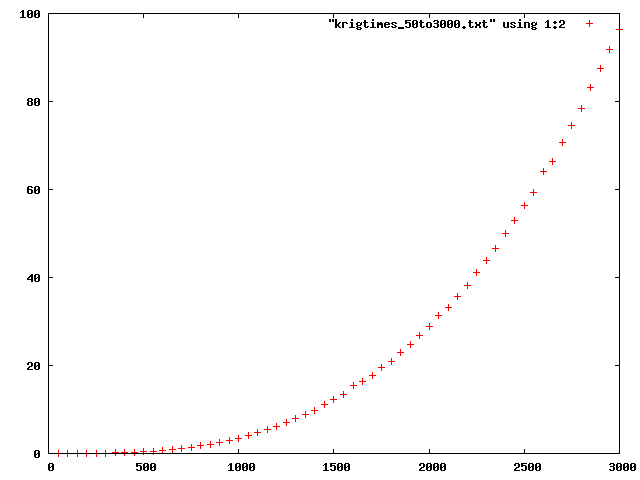
\includegraphics[width=8cm]{TimingMatrixOp/kriging_times_50to3000.png}
  \label{fig:kriging_times}
  \caption {Running times in seconds for the execution of the Kriging algorithm, which is dominated by a matrix inversion, for data sets of size 50 to 3000.} 
\end{figure}

The Kriging algorithm used in Surfpack---for which the running time is
dominated by a matrix inversion operation---was run using 50--3000 data points,
with tests at intervals of 50 points.  If the algorithm is run using $n$
points, the inversion of an $n$-by-$n$ matrix is required.  For each matrix
size, the median time for five runs of the algorithm is reported.  (The
experiments were run when the machine was not heavily loaded with other
processes, but there is still some variation in running times.)

We will use Surfpack to generate an empirical model from these data, which we
can then use to predict running times on problem sizes for which we have not
gathered actual data.  A portion of the data file is shown in Figure~\ref{fig:timing_data_extract}.

\begin{figure}[htbp]
  \centering
  \begin{bigbox}
	\begin{small}
		\verbatiminput{TimingMatrixOp/timing_data_extract.txt}
 	\end{small}
  \end{bigbox}
  \label{fig:timing_data_extract}
  \caption{ Timing data for execution of the Kriging algorithm on data sets with 50--3000 points.}
\end{figure}

This data was gathered for problems using up to 3000 points (which requires the
inversion of a 3000 by 3000 matrix).  After we create a model to fit these data,
we will evaluate the model to predict running times for problems with up to 5000
points.  The first step is to load the data from the file.
\verbatimtabinput{TimingMatrixOp/load.txt}
From the plot of the data, we can see that the trend in the data is definitely
not linear.  We will attempt to fit the data using a quadratic polynomial.
\verbatimtabinput{TimingMatrixOp/create_surface.txt}
We can use Surfpack to generate the set of test data points and then evaluate
the model on those data.
\verbatiminput{TimingMatrixOp/evaluate_and_save.txt}

Figure~\ref{fig:test_data_extract} shows a portion of the output file \texttt{test\_timing\_data.txt}, which
lists the predictions of the model for problem sizes of 50 to 5050, at 100 point
intervals.
\begin{figure}[htbp]
  \centering
  \begin{bigbox}
	\begin{small}
	\verbatimtabinput{TimingMatrixOp/test_data_extract.txt}
 	\end{small}
  \end{bigbox}
  \label{fig:test_data_extract}
  \caption{Timing predictions for quadratic polynomial fit.}
\end{figure}
A plot of the observed data and model predictions is shown in Figure~\ref{fig:timing_poly2}.

\begin{figure}[htbp]
  \centering 
  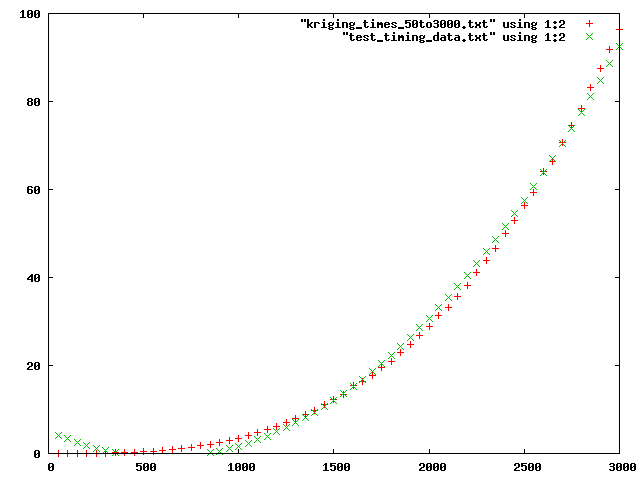
\includegraphics[width=8cm]{TimingMatrixOp/timing_poly2.png}
  \label{fig:timing_poly2}
  \caption{ Measured execution times and quadratic polynomial model predictions for Kriging timing study.}
\end{figure}

Figure~\ref{fig:timing_poly2_extract} shows an excerpt from quad\_poly\_snippet.txt, which shows the
formula for the quadratic approximation.
\begin{figure}[htbp]
  \centering
  \begin{bigbox}
	\begin{small}
	\verbatiminput{TimingMatrixOp/timing_poly2_extract.txt}
 	\end{small}
  \end{bigbox}
   \label{fig:timing_poly2_extract}
   \caption{ Analytic form of quadratic polynomial model. }
\end{figure}
\[ time \approx \hat{f}(numpts) = 1.62x^2 - 0.02x + 5.14 \]
The predictions appear to follow the general trend of the data fairly well.  The
model does curve away from the observed values at the lower-valued data points,
but we are more likely to be concerned about the predictions for larger-sized
problems.

We can use Surfpack's \texttt{Fitness} command to quantify the error between the model
and the data.  We will use the \texttt{mean\_abs} metric as an example, which computes
the absolute value of the difference between each data point used to create the
model and the prediction of the model at that point.  The reported value is the
mean of those residuals.

\verbatimtabinput{TimingMatrixOp/fitness_output.txt}

The value of 1.48 means that, on average, the predicted running time differs
from the reported running time by 1.48 seconds.  

Two other common goodness-of-fit metrics are PRESS and $R^2$.
\verbatiminput{TimingMatrixOp/press_rsquared_results.txt}
PRESS gives an average for what the error would be at each data point, if that
point were not included in building the model.  Values close to zero are more
desirable.  The $R^2$ metric measures the fraction of variance in the model
that can be attributed to the variance in the data.  Values close to 1 are more
desirable.

The plots of the data and/or knowledge of the underlying matrix inversion
algorithm may motivate us to try to fit a cubic polynomial to the data.

\verbatiminput{TimingMatrixOp/cubic_poly.txt}

All of the metrics are worse; this raises some red flags.  In particular, it is
not possible for the $R^2$ value to be lower for a least-squares fit to a
cubic polynomial than for the corresponding quadratic.

The file \texttt{TimingMatrixOp/timing\_poly3.txt} shows the coefficients for the model.

\verbatiminput{TimingMatrixOp/timing_poly3.txt}


\[ time = \hat{f}(numpts) \approx - 0.0007x + 0.1095 \]

The cause of the problem is matrix ill-conditioning.  The range of the problem
sizes is 50--3000, while the running times range from a fraction of a second up
to about 100 seconds.  To address this problem, we scale the data so that data
fall in the range $[0,1]$.

\verbatiminput{TimingMatrixOp/scaled_poly3.txt}

Now all the metrics are improvements over the quadratic fit, which suggests that
the cubic-polynomial more accurately reflects the trends in the data.  In the
absence of any additional information, we would likely use the cubic-polynomial
model to make predictions about running times.

Suppose there were computational resources available to generate a few more data
points.  Running times for problem sizes of 3050--5000 points are given in the
file test\_times.txt.  Now we can evaluate our quadratic and cubic models on
these new data and get a better comparison of their predictive capabilities.

\verbatiminput{TimingMatrixOp/timing3050.txt}

\begin{figure}[htbp]
\centering 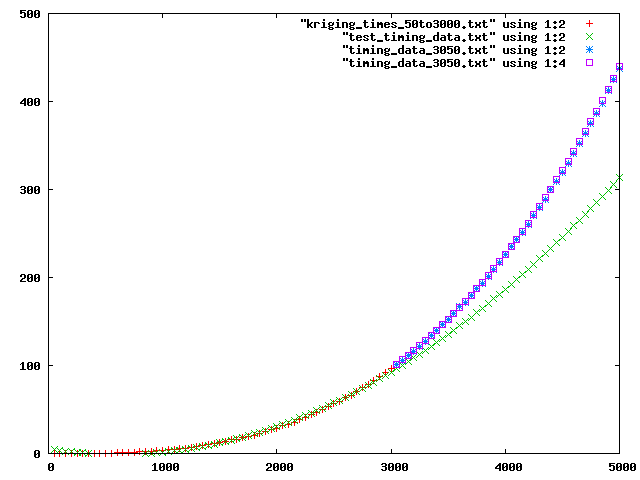
\includegraphics[width=8cm]{TimingMatrixOp/timing_poly2_0to5000_estimates.png}
\end{figure}

The predictions for the cubic-polynomial are impressive.  For a problem size of 5000, the true running time was 437 seconds and the prediction was 439
seconds.

\pagebreak
\subsection {SAT Scores}
The data set in \texttt{examples/TestScores/sat\_scores.spd} give the average Scholastic Achievement Test (SAT) scores, by state, for students during 1982~\cite{powell},~\cite{ramsey}.  The predictor variables for this study were the percentage of the high school seniors taking the test, the median household income for the test takers, the average number of years (in high school) of core courses taken (math, science, English, etc.), the percentage of test takers attending public schools, the average per capita expenditure of the state for education, and the median rank of the test takers in their respective high school classes. 

The script shown in Figure~\ref{fig:test_scores} shows commands that construct several possible models for the data.  The constructed surfaces are saved to files for possible future use.  The PRESS statistic is computed for each model.  The results of the script suggest that the MARS model may have the best predictive capabilities for this application. 
\begin{figure}[htbp]
  \centering
  \begin{bigbox}
	\begin{small}
		\verbatimtabinput[8]{../examples/TestScores/sat_scores.spk}
 	\end{small}
  \end{bigbox}
   \label{fig:test_scores}
\end{figure}

Suppose that education policy makers in Wisconsin wish to use this data to help them get an idea of how their students' SAT scores might be influenced by factors over which they might have some influcence {\em e.g.}, average expenditure per pupil or number of core courses taken in high school.  (Certainly, they should not place too much emphasis on the analysis of this data, since the predictor variables themselves are summaries of many other variables with potentially complicated interactions.  Modeling of this data could be used as one of many tools in a broader analysis.)  

The data \texttt{what\_ifs.spd} include minor variations from the actual Wisconsin data point: an increase in the number of core courses, changes in per pupil spending, etc.  The script \texttt{sat\_scores2.spk} reads in the MARS model that was saved in the earlier script, and then evaluates the model on these specific query points.   

\begin{figure}[htbp]
  \centering
  \begin{bigbox}
	\begin{small}
	\verbatiminput{../examples/TestScores/sat_scores2.spk}
 	\end{small}
  \end{bigbox}
   \label{fig:test_scores2}
\end{figure}

\pagebreak
\subsection {Martian Topology}

Figure~\ref{fig:topology} shows a script that uses both MARS and Kriging to fit data taken from the surface of (the planet) Mars.  The data were sampled from 25--26$^{\circ}$ N latitude and 176--177$^{\circ}$ E longitude. The models are constructed using a sparse training set and then analyzed for their accuracy on both the training set and a more densely sampled test set.  (Data courtesy of NASA.)

\begin{figure}[htbp]
  \centering
  \begin{bigbox}
	\begin{small}
	\verbatiminput{../examples/MartianTopology/mars_terrain.spk}
 	\end{small}
  \end{bigbox}
   \label{fig:topology}
\end{figure}

\pagebreak
\subsection {Sampling Techniques}

This example explores the interaction between sampling method (Monte Carlo, Latin Hypercube, Orthogonal Array) and surface-fitting algorithm (Kriging and MARS) on a commonly used test function, the Rosenbrock ``banana'' function.  Since this is one of Surfpack's built-in test functions, large test data sets are easily created and analyzed.

\begin{figure}[htbp]
  \centering
  \begin{bigbox}
	\begin{small}
	\verbatiminput{../examples/SamplingTechniques/sampling.spk}
 	\end{small}
  \end{bigbox}
   \label{fig:sampling}
\end{figure}

\pagebreak
\subsection {Computational Fluid Dynamics}

\begin{figure}[htbp]
  \centering
  \begin{bigbox}
	\begin{small}
	\verbatiminput{../examples/FluidDynamics/cfd.spk}
 	\end{small}
  \end{bigbox}
   \label{fig:cfd}
\end{figure}

\pagebreak
\subsection {Matlab Peaks Function}

\begin{figure}[htbp]
  \centering
  \begin{bigbox}
	\begin{small}
	\verbatiminput{../examples/MatlabPeaks/peaks.spk}
 	\end{small}
  \end{bigbox}
   \label{fig:peaks}
\end{figure}

\pagebreak
\subsection {Central Composite Design and Latin Hypercube Sampling}

\begin{figure}[htbp]
  \centering
  \begin{bigbox}
	\begin{small}
	\verbatiminput{../examples/Engineering4D/ccd.spk}
 	\end{small}
  \end{bigbox}
   \label{fig:ccd_lhs}
\end{figure}

%\section{Data-fitting algorithms}
%\subsection{Least-squares Polynomial Regression}
%\subsection{Multivariate Adaptive Regression Splines (MARS)}
%\subsection{Kriging Interpolation}
%\subsection{Radial Basis Functions}
%\subsection{Artificial Neural Network}
%

%\section{Test Functions}
%
%\section{Surfpack Library API}
%Brief explanation for writing custom C++ code and linking against the Surfpack library.
%
%\section{Extending Surfpack}
%\subsection{Adding a new surface method}
%\subsection{Adding a goodness-of-fit metric}
%\subsection{Adding a new command-line option}
%
%\section{Using Surfpack with Dakota}
%Brief explanation of how Surfpack fits in with Dakota.  Pointer to Dakota manuals for detailed information about accessing the various options.
%
\section{Troubleshooting}\label{sec:troubleshooting}
List of error messages with probable causes and suggestions for resolving them.

\subsubsection{Bad surface name in file}
When a surface object is read in from a file, the first item listed should be
the name of the surface type (Polynomial, Kriging, etc.) Check to make sure that
the file being read in is indeed a surface file and that it has a valid type
identifier.

\subsubsection{Cannot add another response: the number of new response values does not match the size of the physical data set.}
This happens when some of the points in a data set have been designated as
"excluded."  A list of new response values cannot be added in this state,
because if the currently excluded points were to be included again, they would
not have a needed value for the new response.  Future releases will support
multi-response data setsin which values for some responses may be missing.

To circumvent this problem, activate all points prior to adding a response, or
copy the active points into a new SurfData object, and add the response to the
new set.


\subsubsection{Cannot add response because there are no data points}
The SurfData object to which an attempt is being made to add response data
contains no data points.  The number of points in the data set should correspond
to the number of new response values being added.

\subsubsection{Cannot compute euclidean distance. Vectors have different sizes.}
When computing the distance between two vectors, v1 and v2, make sure that
v1.size() == v2.size().

\subsubsection{Cannot create surface with zero dimensionality}
A query has been made to Polynomial::minPointsRequired in which the
dimensionality of the data set has been declared to be zero.  All data sets must
have dimensionality of at least one.

\subsubsection{Cannot set response index on NULL data }
A response\_index argument has been passed to a Surface object for which the
data set has not yet been specified.  First, specify the data set, using either
the constructor or the setData method.  Then call the config method with an
response\_index Arg object that specifies which response value will be used to
create the surface.

\subsubsection{Cannot specify both data and surface.}
The Save command can be used to write either a data object or a surface object
to a file, but not both.  Specify one or the other.  If both a surface and a
data set need to be saved, use two Save commands.

\subsubsection{Data variable not found in symbol table}
The variable name given for the data argument in a CreateSurface, Fitness, or
Evaluate command was not found in the symbol table.  Make sure that the data
object of that name was previously loaded from a file or created using a
GridPoints or MonteCarloSample command.  Check for misspellings.

\subsubsection{Data unacceptable: there is no data.}
An attempt was made to create a Surface object without specifying any data.
Pass data into the Surface object through the constructor or through the setData
method before invoking createModel.

\subsubsection{Axes variable not found in symbol table.}
The variable name given for the axes argument in a GridPoints or
MonteCarloSample command was not found in the symbol table.  Make sure that the
axes object of that name was previously loaded from a file or created using a
CreateAxes command.  Check for misspellings.

\subsubsection{Dimensionality of data needed to determine number of required samples.}
This error occurs when a request is made to know the minimum number of required
sample for some surfaces before the dimensionality of the data is determined.
In many cases the required number of points is a function of the arity of the
data.

\subsubsection{Dimension mismatch: conmin seed and data dimensionality.}
By default the correlation parameters for Kriging are computed using doing a
maximum likelihood estimation.  If a seed for the optimization is specified, it
should be a tuple with the same dimensionality as the data set.

\subsubsection{Dimension mismatch: correlations and data dimensionality}
Kriging expects one correlation value per dimension in the data set.

\subsubsection{Dim mismatch in SurfData::setFLabels}
The wrong number of labels was given for the data set.  These labels are only
for the response variables.  Use setXLabels to specify tags for the predictor
variables.

\subsubsection{Dim mismatch in SurfData::setXLabels}
The wrong number of labels was given for the data set.  These labels are only
for the predictor variables.  Use setFLabels to specify tags for the response
variables.

\subsubsection{End of file reached unexpectedly.}
When reading data in from a file, there were fewer points than expected in the
file or fewer values for a particular point than were expected.  Please check
the data file.

\subsubsection{Error in dgglse}
The info flag to the LAPACK routine dgglse returned a non-zero value.  See the
LAPACK documentation for details.  The dgglse routine is used in conjunction
with constrained least-squares solves in the PolynomialSurface class.

\subsubsection{Cannot add response because physical set size is different than logical set size.}
Before adding another response, clear excluded points or create a new data set
by using the SurfData::copyActive method.  This inconvenience will be resolved
in future releases.

\subsubsection{Cannot write SurfData object to stream.  No active data points.}
Clear the excluded data points before writing the data to a file.

\subsubsection{Data unacceptable: this surface requires....} 
The various data-fitting algorithms have their own requirements for how many
points are necessary to compute an approximation.  Use the numPointsRequired
method to find how many points are required.  Note that this is only the minimum
number of points for the algorithm to perform its computations.  The number of
points needed to get a model that gives useful predictions may be much, much
greater.  Quantifying these needs is the subject of current research.

\subsubsection{Error in SurfData::addPoint. Points in this data set have....}
The collection of points in a SurfData object must all have the same number of
predictor variables.  Currently, they must also have the same set of response
variables, although this requirement will be relaxed in future releases.

\subsubsection{Error in SurfData::sanityCheck....} 
Surfpack has discovered a mismatch in the dimensionality of at least two data
points in a single SurfData object.  This error can be caused by the
modification of individual SurfPoint objects (through external handles) after
they have been added to a SurfData object.  While there are legitimate uses of
external handles to a SurfData object's data points, care must be taken to avoid
this kind of inconsistency.

\subsubsection{Requested ... max index ....}
A data point was requested from a SurfData object, but the index given is equal
to or greater than the number of points in the set.  Remember that if there are
$n$ points, the indices from those points are $0, 1, \ldots, n-1$.

\subsubsection{Exception caught and rethrown in SurfPoint::readText}
\subsubsection{Exception rethrown in SurfPoint::readBinary}
An unknown error occured while reading a file.  Check the integrity of your
data.

\subsubsection{Expected: \ldots found: \ldots} 
The name found in a surface file is inconsistent with the type of Surface object
that is being create from the file.  Check the file contents and object
constructor.

\subsubsection{Expected `f' or `v' on line}
The first line of an axes object should be the number of dimensions desired in
theresulting data set.  Each line after the first should either give a minimum,
maximum, and number of raster points for one dimension, or it should give a
fixed valuefor a dimension, which all points in the set will share.  Lines with
fixed values should begin with the flag `f'; all others should begin with `v'
(for `variable').
\subsubsection{Index \ldots specified, but there are zero\ldots}
Either a request has been made for a data point in a data set where there are no
active points, or a request has been made for a non-existent response variable.
Remember the if there are $n$ response variables, they are indexed from $0$ to
$n-1$.  When requesting data points from a SurfData object, remember that some
points may be inactive (excluded), which would reduce the maximum valid index.

\subsubsection{In Surface::checkData: No data was passed in}
Data for a surface may be specified in the constructor of a Surface object, or
using the setData method.  If neither of these things occurs before the
createModel method is invoked (either directly or indirectly), this error could
result.

\subsubsection{Integer overflow: number of terms exceeds maximum integer}
There are too many terms in the regression model.  Use a lower-order polynomial
to fit the data or project the data into a lower-dimensional space.

\subsubsection{Must know data arity to use uniform correlation value.}
Kriging allows for the specification that the same correlation parameter should
be used for each dimension, but the number of dimensions must be known in
advance.  Specify the data for the KrigingSurface object before invoking this
method.

\subsubsection{Expected on this line\ldots}
The number of predictor and/or response variables on some line in the data file
does not match the specified number(s) for the file.  Check the format of the
file.

\subsubsection{No axes argument specified.}
A GridPoints or MonteCarloSample command was given, but no axes variable was
specified.  The axes variable must be created in a previous command.  It
specifies the (hypercube) boundaries for the data set, and in the case of the
GridPoints command, the number of raster points per dimension.

\subsubsection{No data argument specified.}
A data argument is required for the CreateSurface and Evaluate commands.  The
data object must have been created (and named) previously in a LoadData,
GridPoints, or MonteCarloSample command.

\subsubsection{No error metric of that type in this class.}
Not all metrics are supported by all methods.  Consider using an alternate
metric or extending Surfpack to support the desired metric.

\subsubsection{No existing surface variable specified.}
The Fitness command requires the name of a Surface object that has already been
created by a LoadSurface or CreateSurface command.

\subsubsection{No filename specified.}
All of the Load and Save commands require a valid file name to be given.  In all
cases, the name of the appropriate argument is `file'.

\subsubsection{No fitness metric specified.}
The Fitness command requires the specification of a metric.  See section xx for
a discussion of supported metrics.  See section xx for an explanation of how to
extend Surfpack with a new metric.  In arguments to the Fitness command, names
of metrics should not be quoted.
\subsubsection{No name argument specified.}
The LoadData, LoadSurface, CreateAxes, CreateSurface, GridPoints, and
MonteCarloSample all create new objects that are to be stored in the symbol
table for future reference.  Each command requires a name argument that gives a
designation to the new entity.

\subsubsection{No surface or data argument specified.}
The Save command expects either a surface argument or a data argument (but not
both).  Check for misspellings.

\subsubsection{No surface type specified.}
The CreateSurface command requires a type argument to specify which algorithm
should be used to approximate the data: polynomial, kriging, mars, ann, or rbf.
See section xx for an explanation of these algorithms.

\subsubsection{Not enough data to compute PRESS.}
If a Surface object is created using the minimum number of required samples,
then the PRESS error metric may not be computed.  PRESS creates the $n$
additional models using the same algorithm, but excluding one of the given
points each time and then predicting the value of that point after the model has
been created.  However, if leaving one point out causes the amount of available
data to fall below what is required, there is no way to compute the metric.

\subsubsection{Out of range in SurfPoint}
The $i$th dimension was requested, but the data has $i$ or fewer dimensions.
Remember that if the data has $n$ dimensions, they are indexed from 0 to $n-1$.

\subsubsection{Size of set of excluded points exceeds size of SurfPoint set}
Some of the indices passed in to setExcludedPoints must either be out of the
range of acceptable indices for the data set, or duplicatations of other
excluded points.

% Surface name not found.
\subsubsection{Surface variable not found in symbol table}
The variable name given for the surface argument in a Fitness or Evaluate
command was not found in the symbol table.  Make sure that the surface object of
that name was previously loaded from a file or created using a LoadSurface or
CreateSurface command.  Check for misspellings.
\subsubsection{There are no response values associated with this point}
A response value has been requested for a data point for which there are no
responses.  If the data were read in from a file, check to make sure the
contents of the file are as expected.

\subsubsection{This Rval class does not have such a value}
This error generally means that the type of an argument in a Surfpack command
was different than what was expected.  Common mistakes are using quoted string
literals where unquoted identifiers are expected (or vice versa), or specifying
a single item when a tuple (a parenthesized list of values) is expected.

\subsubsection{Unrecognized filename extension.  Use .sd or .txt}
\subsubsection{ Unrecognized filename extension.  Use .srf or .txt}
Surfpack uses file extensions to determine the formatting of information that is
read from or written to files.  Currently all Data and Surface files should have
a txt extension.  Future releases will support a binary format for both data and
surfaces.  The binary formats will be more compact and will provide better I/O
performance for large data sets.

% Unrecognized option for surface parameter 'scaling'
\appendix

\section{Surfpack Syntax Summary}
\textcolor{blue}{TODO: Briefly explain the types of arguments: integer, real, identifier, string, list, etc.  In the status column, R means required and O means optional.  Status designations that span multiple rows signify that these arguments are mutually exclusive.}

\begin{table}[h]
  \newcommand\T{\rule{0pt}{2.6ex}}
  \newcommand\B{\rule[-1.2ex]{0pt}{0pt}}
  \centering
  \begin{tabular}{|c|c|c|c|p{8cm}|}
    \hline
    {\bf Command} & \multicolumn{2}{|c|}{\bf Argument}  & {\bf Type} & {\bf Description}  \\ 
    \hline
    \multirow{4}{*}{CreateAxes} & \texttt{name} & R & identifier & unique name for new \texttt{axes} object \\
    \cline{2-5}
    & \texttt{bounds} & \multirow{2}{*}{R} & string & min/max range pairs for each dimension \\
    \cline{2-2} \cline{4-5}
    & \texttt{file} & & string & name of .axb file containing min/max range pairs for each dimension \\
    \cline{2-5}
    & \texttt{labels} & O & identifier list & names for predictor variables in new \texttt{data} object \\
    \hline
   
    \multirow{5}{*}{CreateSample} & \texttt{name} & R & identifier & unique name for new \texttt{data} object\\
    \cline{2-5}
    & \texttt{axes} & R & identifier & existing \texttt{axes} object to be used \\
    \cline{2-5}
    & \texttt{grid\_points} & \multirow{2}{*}{R} & integer list & number of points along each dimension in grid \\
    \cline{2-2} \cline{4-5}
    & \texttt{size} & & integer & number of random samples to draw \\
    \cline{2-5}
    & \texttt{test\_functions} & O & identifier list & names of built-in test functions\\
    \hline

    \multirow{7}{*}{CreateSurface} & \texttt{name} & R & identifier & unique name for new \texttt{surface} object \\
    \cline{2-5}
    & \texttt{type} & R & identifier & surface-fitting algorithm: \texttt{polynomial}, \texttt{mars}, \texttt{kriging}, \texttt{ann} \\
    \cline{2-5}
    & \texttt{data} & R & identifier & existing \texttt{data} object from which to create new \texttt{surface} object \\
    \cline{2-5}
    & \texttt{response} & \multirow{2}{*}{O} & identifier & name of response variable to be used \\
    \cline{2-2} \cline{4-5}
    & \texttt{response\_index} &  & integer & index of response variable to be used \\
    \cline{2-5}
    & \texttt{log\_scale} & O & string list & names of variables to be scaled logarithmically \\
    \cline{2-5}
    & \texttt{norm\_scale} & O & string list & names of variables to be normalized to [0,1] \\
    \hline

    \multirow{3}{*}{Evaluate} & \texttt{surface} & R & identifer & existing \texttt{surface} to be evaluated \\
    \cline{2-5}
    & \texttt{data} & R & identifier & existing \texttt{data} to evaluate \\
    \cline{2-5}
    & \texttt{label} & O & string & name for new response variable \\
    \hline

    \multirow{4}{*}{Fitness} & \texttt{surface} & R & identifier & existing surface to be analyzed \\
    \cline{2-5}
     & \texttt{metric} & R & identifier & goodness-of-fit metric to be used \\
    \cline{2-5}
     & \texttt{data} & O & identifier & existing \texttt{data} object to be used to evaluate fitness \\
    \cline{2-5}
    & \texttt{response} & \multirow{2}{*}{O} & identifier & response variable to be used as ``true'' function value \\
    \cline{2-2} \cline{4-5}
    & \texttt{response\_index} &  & integer & index of response variable to be used \\
    \hline

    \multirow{4}{*}{Load} & \texttt{name} & R & identifier & unique name for \texttt{data} object \\
    \cline{2-5}
    & \texttt{file} & R & string & data file (.spd) or surface file (.sps) \\
    \cline{2-5}
    & \texttt{n\_predictors} & R & integer & number of predictor variables per point (for \texttt{data} load only)\\
    \cline{2-5}
    & \texttt{n\_responses} & R & integer & number of response variables per point (for \texttt{data} load only) \\
    \hline

    \multirow{3}{*}{Save} & \texttt{data} & \multirow{2}{*}{R} & identifier & existing \texttt{data} object \\
    \cline{2-2}
    \cline{4-5}
	 & \texttt{surface} &  & identifier & existing \texttt{surface} object \\ 
    \cline{2-5}
	 & \texttt{file} & R & string & filename for \texttt{data}/\texttt{surface} to be saved \\
    \hline

  \end{tabular}
\end{table}

\pagebreak

\begin{table}[h]
  \newcommand\T{\rule{0pt}{2.6ex}}
  \newcommand\B{\rule[-1.2ex]{0pt}{0pt}}
  \centering
  \begin{tabular}{|c|c|c|c|p{8cm}|}
  \hline
  {\bf Surface Type} & {\bf Argument} & {\bf Status} & {\bf Type} & {\bf Description} \\
  \hline
  Polynomial & order & O & integer & maximum order of regression terms \\
  \hline
  \multirow{3}{*}{Mars} & max\_bases & O & integer & maximum number of basis functions \\
  \cline{2-5}
   & max\_interactions & O & integer & maximum number of interactions between variables per basis \\
  \cline{2-5}
   & interpolation & O & identifier & type of splines used: linear or cubic \\
  \hline
  

  \multirow{3}{*}{Kriging} & correlations & O & real list & correlation paramter for each variable \\ 
  \cline{2-5}
   & uniform\_correlation & O & real & uniform correlation value for all variables \\ 
  \cline{2-5}
   & conmin\_seed & O & real list & starting values maximum likelihood estimation of correlations \\
  \hline 
  
  \multirow{3}{*}{ANN} & norm\_bound & O & real & \textcolor{red}{Does anyone know what this is?}\\ 
  \cline{2-5}
   & svd\_factor & O & real & \textcolor{red}{Does anyone know what this is?}\\ 
  \cline{2-5}
   & fraction\_withheld & O & real & fraction of data to be excluded from training set \\
   \hline 
  \end{tabular}
\end{table}
  
\bibliography{surfpack_users_manual}
\end{document}
 

% LocalWords:  Kriging Surfpack Giunta geostatistics GEK 1derivative order1 spd
% LocalWords:  Sandia executables covariance unadjusted 1order1 nonnegative 1D
% LocalWords:  1reduced polynomial1 Matern differentiable Gneiting et 1powered
% LocalWords:  exponential1 1matern1 1infinity1 differentiability 1optimization
% LocalWords:  method1 1none1 1correlation lengths1 semivariograms
